\documentclass[11pt,a4paper]{article}
\usepackage[utf8x]{inputenc}
\usepackage[T1]{fontenc}
%\usepackage{gentium}
\usepackage{mathptmx} % Use Times Font

\usepackage{graphicx} % Required for including pictures
\usepackage{hyperref} % Format links for pdf
\usepackage[british]{babel} % Multilingual bibliographies
\usepackage{natbib}
\setlength{\bibsep}{0.0pt}

\frenchspacing % No double spacing between sentences
\usepackage[margin=1in]{geometry}

\usepackage[all]{nowidow} % Tries to remove widows
\usepackage[protrusion=true,expansion=true]{microtype} % Improves typography, load after fontpackage is selected

\usepackage{lipsum} % Used for inserting dummy 'Lorem ipsum' text into the template

\usepackage[autostyle]{csquotes} % Adds support for single quotes
\usepackage{amsmath}  % Import alignment facilities
\usepackage{subcaption}  % Import alignment facilities
\usepackage{booktabs}

\newcommand{\ra}[1]{\renewcommand{\arraystretch}{#1}}

\title{Popularity of Munros}
\author{Filip Balucha, Advaith Sai Maddipatla, Tudor Finaru}
%\usepackage{natbib}

\begin{document}

\maketitle

%% INSTRUCTIONS:
%%
%% 1. Please rename this file fds-project-option-1.tex,
%% fds-project-option-2.tex, or fds-project-option-3.tex, depending on
%% which project option you are doing. When you submit, please submit
%% the PDF file with the corresponding name.
%% 
%% 2. You can edit either using:
%%
%%    a. Overleaf professional, a collabaratorive LaTeX editor. See
%%       https://www.overleaf.com/edu/edinburgh for documentation. Create an
%%       empty document, and copy the files in this directory to it.
%%
%%    b. A LaTeX editor on your PC - you can commit changes to this
%%       repository to collaborate.
%% 
%% 3. Please keep the section and paragraph headings as they are.
%%
%% 4. The word limit for the Overview section is mandatory. For the
%% other sections word limits are suggested.
%%
%% 5. The page limits must be strictkly adhered to, and depend on if
%% you are working individually, in pairs or in threes:
%%
%%   - Individual: 6 pages 
%%   - Pairs: 8 pages 
%%   - Threes: 10 pages 
%%

\section{Overview}
% 250 words maximum
Description of problem, work carried out, and results \\ \\ 
This paper answers a few key questions regarding Munro hiking by applying statistical methods on data that is freely available online. It aims to explore the reasons behind the popularity of specific hills, and then provides an appropriate clustering of Munros according to their features. In order to achieve this, we used techniques such as linear regression, principal component analysis, and K-Means clustering. The results from these techniques yielded good results enabling us to reach a number of solid conclusions. First of all, we have established the existence of a statistically significant relationship between Munro altitude and number of ascents. Furthermore, we have managed to identify several other factors that have an influence on Munro popularity – for example the numbers of neighbouring Munros, hotels, and the distance to the nearest city. Finally, we have divided the Munros into four well-defined clusters according to their features.

\section{Introduction}
% Suggested 400 words

\paragraph{Context and motivation}

What is the area of this data science study, and why is it interesting
to investigate? \\ \\
We aim to shed light on the patterns of human behaviour and preferences surrounding Munro hiking – an increasingly popular pastime \cite{CSM}. Many of these hills hold an almost sacred spot in the Scottish psyche, with some locals attaching their very identities to these pieces of timeless, rugged landscape \cite{HAE}. Considering the extensive data on Munros that is available online – as well as the lack of previous scientific literature on the subject – we deemed this topic worthy of further investigation.

\paragraph{Previous work}

Brief description of any previous work in this area (e.g., in the
media, or scientific literature or blogs). \\ \\
There has not yet been a comprehensive study to investigate the patterns that we are trying to observe in this paper. However, there are certainly examples of similar studies carried out about other mountain ranges – a particularly thorough one has been conducted on the Italian Dolomites \cite{HitA}. Among other things, the way the authors 'nested' peaks according to their features has been a useful source of inspiration for our own clustering and linear regression models. 

\paragraph{Objectives}

What questions are you setting out to answer? \\ \\
We are setting out to answer the following questions:
\begin{itemize}
    \item Is there a statistically significant relationship between Munro height and the number of ascents?
    \item What other factors have a significant impact on Munro popularity?
    \item Can Munros be clustered according to their features?
\end{itemize}

\section{Data}
% Suggested 300 words

\paragraph{Data provenance} Who created the dataset(s)?  How you have
obtained it (e.g., file or web scraping), and do the T\&Cs allow you
to use obtain the data for the project? \\ \\
We used three datasets: 
% DECIDED reference T&Cs
\begin{itemize}
    \item WalkHighlands (WH), from which we extracted data on the popularity, rating and accessibility of Munros. This data relies on contributions from registered users – they can select and rate the Munros they have climbed. We retrieved the data using web scraping for the main Munro tables and subpages; additionally, we manually copied the number of facilities for each type of accommodation from the relevant subpages. These methods were chosen after a careful assessment of the T\&Cs.
    \item The Database of British and Irish Hills (DoBIH), from which we extracted geographical data on the Munros. The origins of this data can be traced in a \textquote{series of articles in Marhofn and Relative Matters magazine}, according to the website. The current editorial team consists of Graham Jackson, Chris Crocker, John Barnard, Simon Edwardes, George Gradwell, Jim Bloomer, and Dave Marshall. The T\&Cs of this dataset are quite liberal, as they impose \textquote{no restrictions on use of the data by third parties}, so long as the terms of the Creative Commons license are respected. Retrieving the data was easy, as it only involved downloading a readily available CSV file.
    \item Simplemaps Cities Database (SCD), from which we extracted data on British cities' location and population. The data comes from the US National Geospatial-Intelligence Agency, and is freely available to use under the MIT license. Again, retrieving the data only involved downloading a CSV file.
\end{itemize}
% DECIDED Put into paragraph as opposed to list
All web scraping was performed in accordance with James Densmore's rules for ethical web scraping \cite{EiWS}:
\begin{itemize}
    \item We only scraped data when necessary – i.e. if no file or API was accessible.
    \item We always provided a “User Agent” string to make our intentions clear to the site owner, as well as to provide a way to contact the team member responsible for data processing.
    \item We requested data at a reasonable rate of at most 1 request per 10 seconds.
    \item We only saved the data we absolutely needed.
    \item We respected all data we obtained, and we did not pass it off as our own.
\end{itemize}

\paragraph{Data description} Description of the data, e.g. variables
in each table, number of records. \\ \\
After processing the data and joining the resulting tables (see \textquote{Data processing} for details), we obtained a data set with 282 records and variables as outlined Table~\ref{table:1}.
% TODO: reference the section?

\begin{table}
    \centering
    \begin{tabular}{l  l  l} 
        \toprule
        Variable & Type & Description  \\ 
        \midrule
        name & string & Name of the Munro \\ 
        altitude & integer & Altitude of the Munro [m] \\
        \hline
        rating & float & Normalised rating on a scale of 0 to 5 by WH users\\
        rating\_count & integer & Number of ratings for the Munro \\
        ascent\_count & integer & Number of ascents by WH users\\
        report\_count & integer & Number of reports from WH users for the Munro\\
        \hline
        region & string & Region in which the Munro is located \\
        county & string & County in which the Munro is located\\
        island & string & Island on which the Munro is located\\
        latitude, longitude & float & Coordinates of the Munro's peak\\
        \hline
        bb\_count & integer & Number of B\&Bs in the region\\
        hotel\_count & integer & Number of hotels in the region\\
        hostel\_count & integer & Number of hostels in the region\\
        cottage\_count & integer & Number of cottages in the region\\
        camping\_count & integer & Number of camping and glamping sites in the region\\
        \hline
        nearest\_city\_dist & float & Distance to the city closest to the Munro [km]\\
        nearest\_city\_population & integer & Population of the city closest to the Munro\\
        %  \hline 
        %  nearest\_large\_city\_dist & float (2 d.p.) & Distance to the nearest large city in kilometres\\
        neighbor\_count\_<$r_1$>\_<$r_2$> & integer & Number of neighbouring Munros within $(r_1,r_2]$ km\\
        population\_<$r_1$>\_<$r_2$> & integer & Population within $(r_1,r_2]$ km\\
        \bottomrule
    \end{tabular}
    \caption{The variables present in the final data set.}
    \label{table:1}
\end{table}
% TODO: group variables?
% TODO: use actual vaulues instead of r_1 and r_2? ('neighbor_count_0_5', 'neighbor_count_5_20', 'population_0_25', 'population_25_50', 'population_50_75', 'population_75_100')
% TODO: add? 'beginner_friendly', 'national_park', or 'nearest_large_city_distance'
\paragraph{Data processing} How you have processed the dataset, e.g.,
cleaning, removing missing values, joining tables.\\ \\
% DECIDED clarify bayesian average
% After scraping the WH data, we normalised the ratings since the rating count presented wild variations (taking values between 22 and 317). We computed the Bayesian average, which pulls ratings that are based on few votes closer to the mean rating. It uses two fields: $m$, the prior mean, i.e. the mean rating for all Munros, and $C$, the number of ratings required for a decent estimate of the sample mean. In other words, $C$ is the number of observations necessary to “get away” from $m$. These values were determined using a joint distribution plot of “rating” and “rating\_count” to be $m = 3.6$ and $C = 60$. \\ \\
% TODO: variable format
For the DoBIH data, we only chose the Munros. We kept only the relevant columns, which were name, altitude, island, county, and its latitude and longitude. \\ \\
For the SCD data, we first filtered out cities not in the UK. Then, for each Munro, we computed the distance to and population of the nearest city, as well as the distance to the nearest large city. We considered any city with a population of at least 50,000 to be large, since the 10 largest Scottish cities fulfill this criterion. To represent the various distances from which hikers come, we also computed the total population within increasing ranges of distances from the Munro.\\ \\
We treated the islands of Mull and Skye separately, since neither Portree nor Tobermory, their corresponding largest settlements, are in the database. Considering that Skye is connected to the mainland via a road bridge, we considered the impact of mainland cities on the popularity of Skye Munros. However, since Mull is isolated from the mainland, we simply replaced all city-related values with NaN. \\ \\
Merging the WH and DoBIH datasets was challenging. First, we created a unique key for each Munro in both tables. The key of choice was a stringified tuple consisting of name and altitude, since only these two fields are available in both datasets. Sadly, they did not always match exactly - some particular cases were so bad that they needed to be handled manually (e.g. the name “Carn Dearg” appears in DoBIH three times). For the remaining data, we performed fuzzy matching on the keys i.e. we matched a key from WH to the closest key in DoBIH based on string edit-distance. We verified the matched key pairs by flagging any pair for which the difference in altitudes was greater than 10m (i.e. greater than $\approx1\%$ of 1018m – the mean Munro altitude) or if the intersection of their names did not match either name. We also ensured that all keys were unique. We then merged the data and removed unnecessary fields such as the aforementioned keys. \\ \\
After merging, we computed the number of \textquote{neighbours} for each Munro, that is, the number of Munros located within a \textquote{ring} comprising areas located between 0 and 5 km away, and 5 and 20 km away. The former represents Munros that could be reached on foot as part of a single trek, while the latter other Munros that are within driving distance and could be visited during a single trip. We only considered neighbouring Munros located on the same land mass, since we assume that a climber who is to climb multiple Munros in a restricted area will not want to drive to another island to do so (e.g. Skye).

% TEMP dash: –

\section{Exploration and  analysis}
% Suggested 500 words for individual report; proportionately longer
% for group projects).

% DECIDED: no need for "as seen in Figure x" afaik it's preferable to use (Figure x) if possible

% DECIDED: add caption for (a), (b) (https://tex.stackexchange.com/questions/211748/multiple-captions-under-a-single-figure)
\subsection{Assessment of the statistical significance of the relationship between Munro height and the number of ascents}
To get an initial view of the data, we start by visualising the distributions of Munro ascent counts and heights (Figure~\ref{fds-project-template:fig:box_dist}). We observe that most Munros have been ascended 2500 to 3000-times. The associated box plot tells us that an ascent count greater than 11,000 is an outlier (Figure~\ref{fds-project-template:fig:box_dist_ascents}). . We also notice that most Munros have an altitude just below 1000m, with any Munro higher than $1,230$m being an outlier (Figure~\ref{fds-project-template:fig:box_dist_altitude}).
% TODO finish comment on outliers: There exist a number of apparent outliers in the data – as was also visible in the boxplots attached to Figure~\ref{fds-project-template:fig:box_dist}.

% TODO: bin sizes! values are still hard to read off!
% TODO: 2.5 really won't fit in figure 1
\begin{figure} [h!]
    \centering
    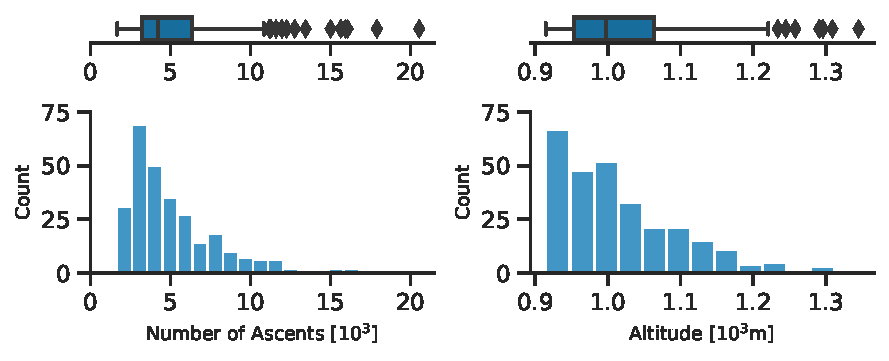
\includegraphics{report/box_dist.pdf}
    \begin{minipage}[t]{.5\linewidth}
        \centering
        \subcaption{The distribution of number of ascents.}
        \label{fds-project-template:fig:box_dist_ascents}
    \end{minipage}%
    \begin{minipage}[t]{.5\linewidth}
        \centering
        \subcaption{The distribution of Munro altitude.}
        \label{fds-project-template:fig:box_dist_altitude}
    \end{minipage}
    \caption{The distributions for number of ascents and altitude.}
      \label{fds-project-template:fig:box_dist}
\end{figure}
In order to better understand and identify some key outliers, it is worth having a look at a scatterplot of ascent count and altitude (Figure~\ref{fds-project-template:fig:scatterplot}). It comes as little surprise that the two most popular Munros are Ben Lomond and Ben Nevis. In fact, Ben Lomond takes the top spot despite being less than 1000 metres high. This could likely be explained by its extraordinary popularity with the people of Glasgow, Scotland's most populous city. It is within easy reach of said city, and is well-known as an accessible spot of natural beauty for Glaswegians. On the other hand, Ben Nevis' significant popularity was expected given its status as the tallest mountain in Britain. Its relatively isolated location in the North-West of Scotland does little to deter plenty of people from all over the UK from attempting the comparatively strenuous hike. \\ \\
% TODO: comment on the different scale in x and y-axis
% TODO: y-axis from 0
\begin{figure} [h!]
  \centering
  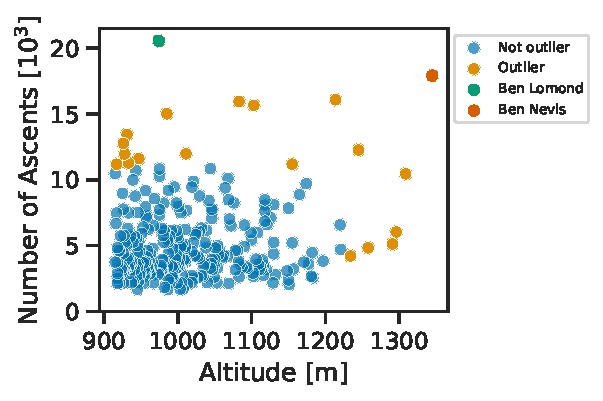
\includegraphics{report/scatterplot.pdf}
  \caption{Scatterplot of ascent count and altitude with key outliers highlighted.}
  \label{fds-project-template:fig:scatterplot}
\end{figure}

We are now in a better position to answer our initial question. Judging by Figure~\ref{fds-project-template:fig:scatterplot}, there appears to be no clear relationship between Munro altitude and ascent count. However, the outliers (e.g. Ben Nevis) should exert a leverage and thus we can still expect to see a positive relationship between number of ascents and altitude. Nevertheless, our conclusions will unfortunately be marred by the large variance in the left-hand side of the scatterplot. \\ \\
We use hypothesis testing. The null and alternate hypotheses are as follows:
% DECIDED: change null hypothesis to: hypothesis that 
%  this matches what's used by statsmodels, so could be less confusing
\begin{align*}
    H_0 &= \text{There is not a statistically significant relationship between altitude and number of ascents.}\\
    H_\text{a} &= \text{There is a statistically significant relationship between altitude and number of ascents.}
\end{align*}
% DECIDED explain why log transform
% TODO: fix transition here
Before applying Ordinary Least Squares (OLS) linear regression we need to make sure that our dependent variable is not highly skewed. In order to see if that is the case, we plot the distribution of Ascent Count and notice that it is right-skewed. In order to fix this skew, we log-transform Ascent Count. This yields a distribution which is less skewed and which looks approximately normal (Figure~\ref{fds-project-template:fig:ascent_count_distribution}).
% DECIDED: Split into figure a and b
% TODO: need left hand side plot? since already in fig 1a...
% TODO: right hand side: more space aaround, better x-axis numbering
% TODO: should use shared y-axis? x-axis may be a bit misleading, b is actually much more "normal"
\begin{figure} [h!]
  \centering
  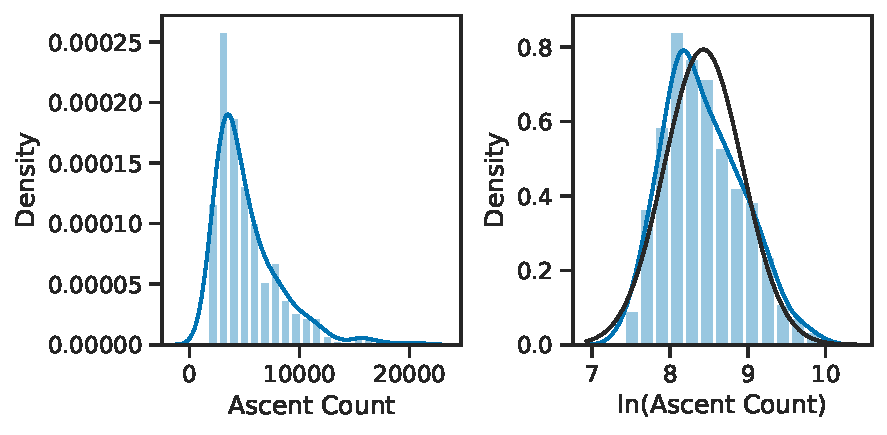
\includegraphics{report/ascent_count_distribution.pdf}
  \begin{minipage}[t]{.5\linewidth}
        \centering
        \subcaption{The distribution of number of ascents.}
        \label{fds-project-template:fig:box_dist_ascents}
    \end{minipage}%
    \begin{minipage}[t]{.5\linewidth}
        \centering
        \subcaption{The distribution of log-transformed number of ascents.}
        \label{fds-project-template:fig:box_dist_altitude}
    \end{minipage}
  \caption{The distribution of Ascent Count before and after log-transformation.}
  \label{fds-project-template:fig:ascent_count_distribution}
\end{figure}
% DECIDED: remove error message: reword in human language
% TODO: not sure if OLS can be used to denote linear regression - OLS has different, well-defined meaning, after all
Upon applying OLS, statsmodels alerts us about numerical instability. We remedy it by normalising the independent variable – i.e. centering it around 0. Applying OLS on the processed data yields the prediction seen in Figure~\ref{fds-project-template:fig:q1_prediction}.
\begin{figure} [h!]
  \centering
  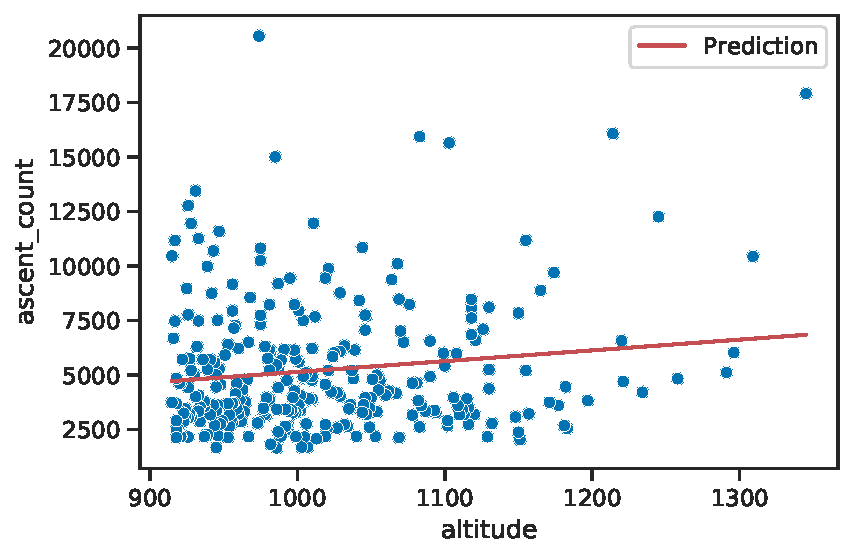
\includegraphics{report/q1_prediction.pdf}
  \caption{Prediction over centered data}
  \label{fds-project-template:fig:q1_prediction}
\end{figure} \\ \\
% DECIDED explain why 5%
Again, we note some important results from statsmodels. The $p$-value tells us that there is a $\approx 3.4\%$ probability that the relationship between altitude and ascent count may be due to chance. Since $0.034 < 0.05$, it allows us to reject the null hypothesis that the coefficient of altitude in the model equals 0 at the $5\%$ level. Furthermore, the t score is fairly high too, which further asserts our claim. Thus, there is a statistically significant relationship between altitude and ascent count. However, we observe that the $R^{2}$ value is quite low at $0.016$. This tells us that the model does not explain the variance in the data too well. This motivates the use of further predictors to aid our analysis.

Since we normalised the independent variable, it has mean 0. Thus for the mean Munro, $\ln$(Ascent count) is equal to the intercept. This tells us the expected ascent count for a Munro of mean altitude is $e^{\beta_0}=e^{8.4286}\approx 4576$ ascents. To understand the meaning of the slope $\beta_1$, we note that the linear regression is of the form $\beta_0 + \beta_1x = \ln(y)$ so that $\beta_0 + \beta_1x = \ln(y_1)$ and $\beta_0 + \beta_1x = \ln(y_2)$ for two observations. Then $\beta_1(x_2 - x_1) = \ln(y_2) - \ln(y_1) = \ln(y_2 / y_1)$. Now for a unit increase in the dependent variable we have $x_2 - x_1 = 1$, and finally $e^{\beta_1} = y_2 / y_1$, which can be rewritten as $e^{\beta_1} - 1 = (y_2 - y_1) / y_1$. Thus, a unit increase in altitude leads the ascent count to increase by $100(e^{0.0008} - 1)\% \approx 0.08\%$. The confidence interval tells us that in $95\%$ of all samples that could be drawn, $[5.57 \times 10^{-5}, 0.001]$ will include the true value of the coefficient for altitude, i.e. that the increase in ascent count will be within $[0.00570, 0.100]\%$.\\ \\
An assumption of linear regression is that the residuals are normally distributed. This appears to be the case, as seen in Figure~\ref{fds-project-template:fig:uni_residuals}. Furthermore, there is no obvious pattern observed – the independent variable and variance do not exhibit a relationship. 
% DECIDED refer to right hand plot in Figure 5
Thus, the plot is not heteroskedastic. Therefore, the linear model that we used earlier was a reasonable choice for the given task.\\ \\
% DECIDED: captions for a and b, fix discussion accordingly
\begin{figure} [h!]
  \centering
  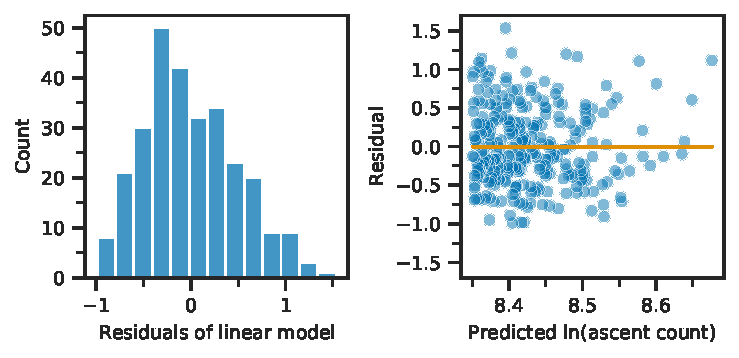
\includegraphics{report/uni_residuals.pdf}
  \caption{Residuals}
  \label{fds-project-template:fig:uni_residuals}
\end{figure} \\ \\
% DECIDED: what is the question?, remove reference to question
\subsection{TBA}
Moving on to our second question, we need to perform some feature selection on our data. The technique we will be using only expects continuous data, so we ignore the columns with categorical or boolean values. In addition, we ignore rating\_count, since it is not an inherent property of a Munro, and learning about its importance would not provide useful insight. \\ \\
Now that we have our subset data with all relevant features, we standardise the dataset. This helps with numerical stability because some features have a vastly different range of values (e.g. population can be in the thousands, whereas hotel\_count is in the tens). \\ \\
We use scikit-learn's SelectKBest class to select features. We score the features using the scoring function f\_regression, which is equivalent to running a univariate linear regression test for each independent variable. According to the official documentation \cite{scikit-learn}, f\_regression first computes the Pearson correlation coefficient between the regressor and the target. It outputs a $p$-value, which corresponds to the null hypothesis that there is no linear interaction between between the regressor and the target. We pick the regressors whose $p$-value falls below a certain threshold. As in the previous section, we choose the threshold to be 0.05, such that the null hypothesis can be rejected at the $5\%$ level. That is, we pick only those regressors for which there is a $5\%$ probability that the linear interaction with the target is due to chance. \\ \\
Before we apply multivariate OLS linear regression, we ensure that there is not significant multicollinearity between our features since that could negatively affect numerical stability, and hence jeopardise the quality of our prediction. To this end, we inspect the correlation matrix for the selected independent features. All correlation coefficients are below 0.8, and so we do not need to remove any features. \\ \\
We now apply OLS regression. We will use each of the standardised features as regressors. The target will be the log-transformed Ascent Count, for the same reason as in previous section. We find that the variables population\_25\_50 and hostel\_count both have quite high $p$-values of over 0.2. This is likely due to multicollinearity with other population- and accommodation-related features, and it is therefore safe to remove these. \\  \\
% DECIDED: explain F-statistic or remove it
After reapplying OLS, we obtain a good fit with an adjusted $R^{2}$ of 0.525 and an $F$-statistic of 45.39. In addition, we notice that all the features in model have a $p$-value of less than 0.01. This indicates the obtained coefficients are reliable. \\  \\
We now wish to interpret the output of statsmodels. Since the regressors are standardised and the target is log-transformed, we first need to transform them to an interpretable format. We are interested in the impact of a unit change in a regressor on the target. The linear regression is of the form 
$$\beta_0+\beta_1z^{(1)}+ \dots + \beta_n z^{(n)}=\ln(y)$$ 
where $z^{(i)}$ is the standardised $i$-th regressor. To interpret the response in the target to a unit increase in the $i$-regressor, we let $x^j = 0, (\forall j \neq i)$. Then we have $\beta_0 + \beta_i z^{(i)} = \ln(y)$. Now $\beta_i (z_2^{(i)} - z_1^{(i)}) = \ln(y_2) - \ln(y_1)=\ln(y_2/y_1)$. Since 
$z^{(i)} = (x^{(i)} - \overline{x}^{(i)})/\sigma_{x^{(i)}}$
due to standardisation, we may rewrite the above as $(\beta_i (x_2^{(i)} - x_1^{(i)}))/\sigma_{x^{(i)}} =\ln(y_2/y_1)$. Skipping steps similar to those in previous section, we arrive at $\exp(\beta_i / \sigma_{x^{(i)}}) - 1 = y_2 / y_1 - 1 = (y_2 - y_1) / y_1$. \\ \\
This result means that a unit increase in an original feature leads to a $100[\exp(\beta_i / \sigma_{x^{(i)}}) - 1]\%$ increase in Ascent Count; we use this value to transform our coefficients accordingly; the results can be seen in Table~\ref{table:2}.
% DECIDED: use scientific notation / at least try
% DECIDED: FILIP: add std for each variable? since used to calculate percentage response in independent variable
\begin{table} [h!]
\centering
\caption{Interpretation of Transformed Coefficients}
\begin{tabular}{|l|l|l|l|}
\toprule
               Feature &  Coefficient &  CI Lower &  CI Upper \\
\midrule
              Altitude &       0.0874 &    0.0376 &     0.137 \\
           Hotel Count &       -0.708 &    -0.984 &    -0.432 \\
Neighbour count 5–20km &        -1.31 &     -1.81 &    -0.805 \\
    Nearest City Dist. &       -0.512 &    -0.888 &    -0.135 \\
            Pop 0–25km &      0.00255 &   0.00132 &   0.00378 \\
           Pop 50–75km &     $0.327 \times 10^{-4}$ &  0.0000242 &  0.0000411 \\
          Pop 75–100km &     0.0000353 &  0.0000281 &  0.0000425
\bottomrule
\label{table:2}
\end{tabular}
\end{table} \\
% TODO: altitude -> Altitude, ascent count -> Ascent Count everywhere?
The intercept gives the expected value of Ascent Count on a log scale when all regressors are 0. The intercept is 8.4286 which implies the expected number of ascents is then $e^{8.4286} \approx 4576$ ascents. \\ \\ 
The most dominant feature is neighbor\_count\_5\_20. Every extra neighbouring Munro within 5-20km reduces the Ascent Count by $ \approx 1.3\%$. The other dominant features are the number of hotels, wherein each extra hotel reduces Ascent Count by $\approx 0.71\%$, and the distance to the nearest city, such that each extra kilometer distance leads to a $\approx 0.5\%$ decrease in Ascent Count. As implied by the first section, altitude also has an impact on ascent count, albeit smaller. Namely, each meter of altitude increases Ascent Count by $\approx 0.87\%$. There is also a slight positive impact on Ascent Count associated with population within 0-25km and 50-100km. \\ \\
We now plot the residuals of our fit against the predictions, as well as the distribution of our errors. As can be seen in Figure~\ref{fds-project-template:fig:multi_residuals_dist}, our errors are normally distributed, which is an assumption of linear regression, and there is no heteroskedasticity exhibited either.
% TODO: missing final sentence -> what this means: linear model is a good choice!
% DECIDED: distplot -> histplot (David's advice!)
\begin{figure} [h!]
  \centering
  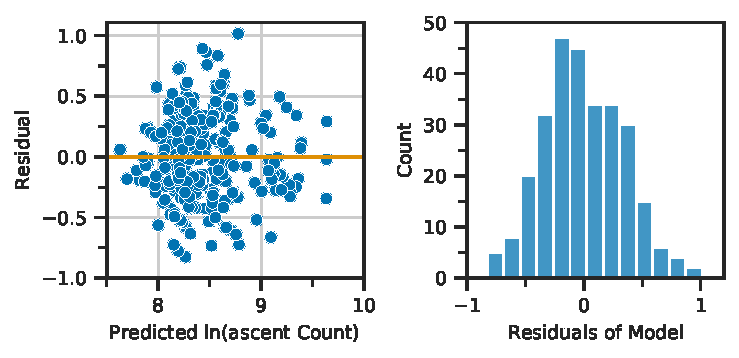
\includegraphics{report/multi_residuals_dist.pdf}
  \caption{Distribution of Residuals}
  \label{fds-project-template:fig:multi_residuals_dist}
\end{figure} \\ \\
% TODO: somehow delimit this section? e.g. new subsection?
% TODO: explain why we look for the knee?
Moving on to our final question, we aim to cluster Munros according to the independent features. This may help us discover a sub-structure within the dataset and help us understand it better. \\ \\
Before performing K-Means Clustering, we need to reduce the number of independent vectors. This is because as a distance-based method, K-Means suffers from the \textquote{curse of dimensionality} and will perform poorly when applied to a vast dataset. Hence, we perform PCA on the dataset. In order to determine the appropriate number of components to be used, plot a scree plot to find the knee. Figure~\ref{fds-project-template:fig:scree_plot} shows that the first 3 principal components help explain a considerable amount of variance. Using the cumulative plot, we see that this is about $60\%$ of the variance. We thus transform the dataset using the first 3 principal components.
% TODO: split into a and b!!!
\begin{figure} [h!]
  \centering
  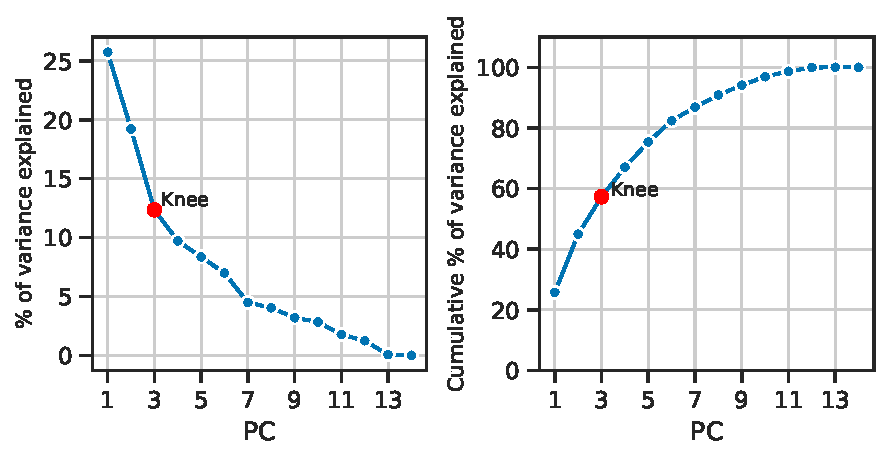
\includegraphics{report/scree_plot.pdf}
  \caption{Scree plot}
  \label{fds-project-template:fig:scree_plot}
\end{figure}
\begin{figure} [h!]
  \centering
  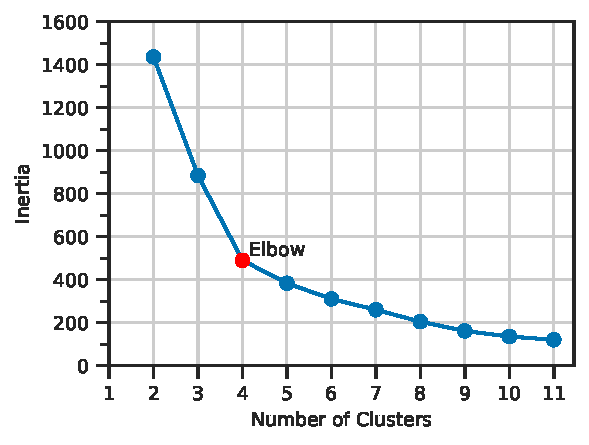
\includegraphics{report/k_screeplot.pdf}
  \caption{K Scree plot}
  \label{fds-project-template:fig:k_screeplot}
\end{figure} \\ \\
% TODO: explain why elbow?
In order to determine the appropriate number of clusters, we inspect the inertia (i.e. the sum of squared errors) of our K-Means model with increasing number of clusters, as can be seen in Figure~\ref{fds-project-template:fig:k_screeplot}. There is a clear elbow at $k = 4$. Thus, the optimal number of clusters is 4. We now perform K-Means. Since we cluster in 3 dimensions, we plot the predictions on a 3D plot and indicate the clusters' centroids (see Figure~\ref{fds-project-template:fig:3d_clusters}). We now use the information about clusters to inspect the features that contribute to each cluster. To obtain a summary measure for each feature, we take the mean of each feature for each cluster. \\
% TODO: better caption (in fact, we should make sure all captions are perfect just in case)
% TODO: make smaller?
\begin{figure} [h!]
  \centering
  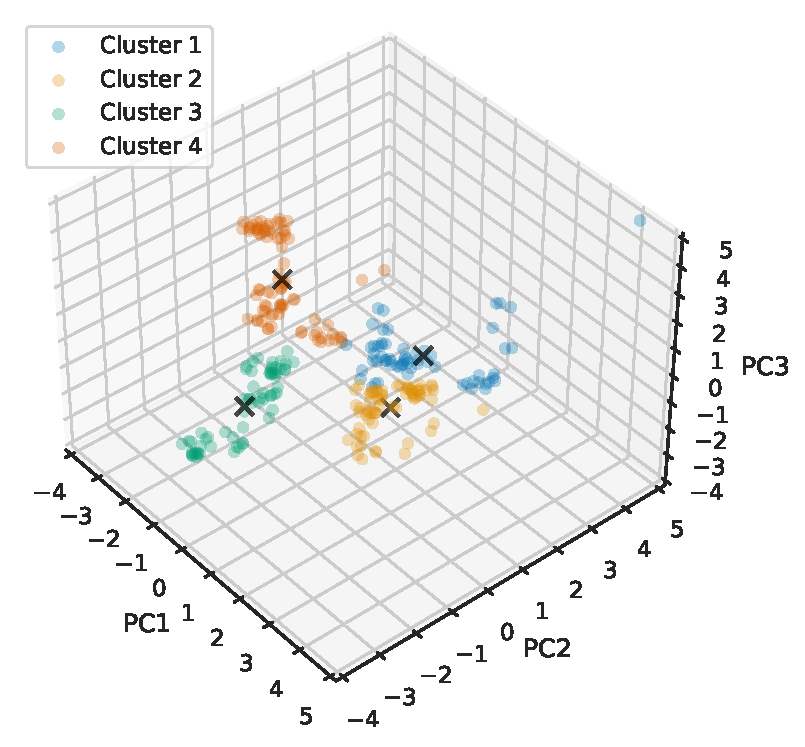
\includegraphics{report/3d_clusters.pdf}
  \caption{Clusters}
  \label{fds-project-template:fig:3d_clusters}
\end{figure} \\
% TODO: settle for either ~ or \approx and use consistently throughout
% TODO: fix hyphen: –
The average Munro in Cluster 1 has $\approx 2000$ inhabitants within 25km, while the nearest city has $\approx 10,000$ inhabitants and is $\approx 35$km away. This cluster has the largest population 25-100km away out of all clusters. At about 60, it also has the largest number of hotels. It also has a fair amount of bed and breakfast accomodations (about 50). It also has the lowest the number of neighbouring Munros: slightly above 2. Since there are very few neighbouring Munros and there are a lot of (presumably relatively high-end) hotels near these Munros, we expect this cluster to comprise of fairly \textquote{exclusive} Munros which are suitable for visitors from a larger city (which makes them quite popular, too). Two examples of Munros that fall into this category are Ben Lomond and Ben Lawers.\\ \\
The average Munro in Cluster 2 does not have a large city within 100km. The nearest city is about \textasciitilde 45km away with a population slightly higher than \textasciitilde 7,500. The dominant accommodation type for this cluster are cottages and camping sites, and there are relatively few B&Bs, hotels and hostels. It has about 25 neighboring Munros within 20km. We are therefore dealing with a region with a fairly high number of Munros, with relatively few accommodation facilities and also quite far away from any major cities. Munros that belong to this cluster are fairly isolated and slightly less popular - two examples would be Mount Keen and Ben Hope. \\ \\ For the average Munro in Cluster 3, the closest city is more than 50km away, but has \textasciitilde 20,000 people – the most across all clusters. It has the largest number of cottages and campings out of all clusters, with relatively fewer B&Bs, hotels and hostels. At more than 4, it also has the largest number of neighboring Munros within 5km. Visitors to Munros included in this cluster might wish to hike several neighboring peaks during their trip and stay at a cottage or camping site. At \textasciitilde 6000 ascents, these Munros are fairly popular – perhaps some inhabitants of the nearby large city are regular visitors, or the high concentration of nearby Munros makes the entire area a popular hiking destination. The latter point is supported by the inclusion of peaks such as Cairn Gorm and The Cairnwell in this cluster; both of these are located in the Cairngorms Natural Park, one of Scotland's prime areas for hiking.\\ \\
The average Munro in Cluster 4 has the largest number of people within 25km across all clusters, but relatively few people beyond that. The nearest city is \textasciitilde 25km away and has a population of about 10,000. Other larger settlements lie beyond 75km away. The dominant accommodation types are B&Bs and hostels. At almost 25, it has the largest number of neighboring Munros within 5-20km. Two examples of peaks that belong to this cluster are Ben Nevis and Stob Dearg; these are both located near Fort William and Glencoe in North-West Scotland, an area famous for its high concentration of dramatic Munros – which certainly ensures a large number of neighboring peaks. Apart from a few minor nearby towns that also present a number of accommodation facilities, Munros in this cluster seem to be quite isolated compared to others – and this definitely applies to the two aforementioned examples. \\ \\
Our conclusions should mostly be trustworthy; however, the nature of the data might affect their accuracy somewhat. Perhaps the most important thing to note is that we are working with the number of ascents by separate individuals as opposed to the frequency of climbs. Additionally, the data on the number of ascents has only been gathered from a single source – and WalkHighlands requires users to register before allowing them to contribute. This means that the group of people who contributed to the data we are using might not be fully representative of all hikers. The contributors can be expected to be active internet users with a real passion for hiking – which is not necessarily the case for every Munro climber.
% 't' means "try to position at the top of the page"
%\begin{figure}[t]
%  \centering
%  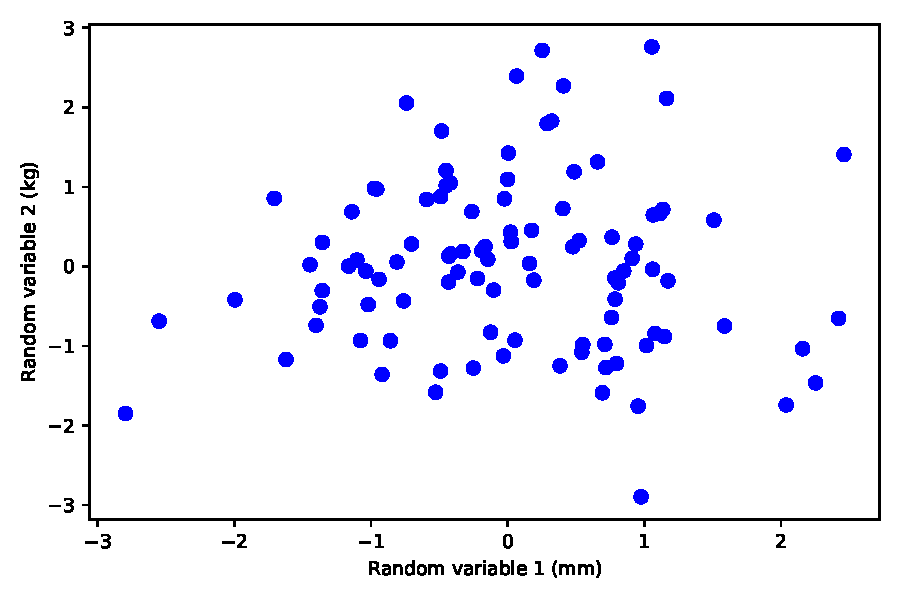
\includegraphics{example1}
%  \caption{Demonstration figure. This caption explains more about the
%    figure. Note that the font size of the labels in the plot is 9pt,
%    which is obtained by the settings as shown in the Jupyter
%    notebook.}
%  \label{fds-project-template:fig:example1}
%\end{figure}

% 'b' means "try to position at the bottom of the page"
\begin{table}[b]
  \caption{Exerpt from Scottish Index of Multiple Deprivation, 2016 edition.
    \url{https://simd.scot}. You may put more information in the caption.}
  \label{tab:example1}
\begin{tabular}{lrrrrrrr}
\hline\hline
\textbf{Location}&\textbf{Employ-}&\textbf{Illness}&\textbf{Attain-}&\textbf{Drive}  &\textbf{Drive}    &\textbf{Crime}&\dots\\
                 &\textbf{ment}   &                &\textbf{ment}   &\textbf{Primary}&\textbf{Secondary}&              &\\
\hline
\textbf{Macduff}&$10$&$ 95$&$5.3$&$1.5$&$6.6$&$249$&\dots\tabularnewline
\textbf{Kemnay}&$ 3$&$ 40$&$5.3$&$2.4$&$2.4$&$168$&\dots\tabularnewline
\textbf{Hilton}&$ 0$&$ 10$&$6.3$&$2.2$&$3.0$&$144$&\dots\tabularnewline
\textbf{Ruchill}&$ 8$&$130$&$4.9$&$1.7$&$5.6$&$318$&\dots\tabularnewline
\textbf{Belmont}&$ 2$&$ 50$&$6.1$&$3.1$&$3.2$&$129$&\dots\tabularnewline
\dots&\dots&\dots&\dots&\dots&\dots&\dots&\dots\tabularnewline
\hline
\end{tabular}
\end{table}

%A data science analysis of the paper, including: 
%\begin{itemize}
%\item Visualisations (for example
%  Figure~\ref{fds-project-template:fig:example1}) and tables (for
%  example Table~\ref{tab:example1}). Please make sure that all figures
%  and tables are referred to in the text, as demonstrated in this
%  bullet point.
%\item Interpretation of the results 
%\item Description of how you have applied one ore more of the
%  statistical and ML methods learned in the FDS to the data
%\item Interpretation of the findings 
%\end{itemize}

%You can use equations like this:
%\begin{equation}
%  \label{fds-project-template:eq:1}
%  \overline{x} = \sum_{i=1}^n x_i
%\end{equation}
%or maths inline: $E=mc^2$. However, you do not need to reexplain %techniques that you have learned in the course -- assume the reader %undertands linear regression, logicstic regression K-nerest neighbours %etc.  Remember to explain any symbols use, e.g.~``$n$ is the number of %data points and $x_i$ is the value of the $i$th data point.''.

\section{Discussion and conclusions}
% Suggested 400 words.

\paragraph{Summary of findings}

\paragraph{Evaluation of own work: strengths and limitations}

\paragraph{Comparison with any other related work}
E.g. ``Anscombe has also demonstrated that many patterns of data can
have the same correlation coefficient'' \cite{Ansc73Grap}.

\paragraph{Improvements and extensions}

\bibliographystyle{unsrt}
\bibliography{fds-project}
\end{document}
